\فصل{تئوری مسئله}
\label{ch:theory}

\قسمت{مدل فیزیکی جریان حامل و حرکت ذره}
\label{sec:theory-physical-model}

برای پیش‌بینی مسیر ذره، ابتدا میدان سرعت سیال را مشخص می‌کنیم.
ذره در هر لحظه با سرعت سیال در مکان خودش برهم‌کنش دارد.
اثر این برهم‌کنش با نیروی درگ در معادلهٔ حرکت وارد می‌شود.
در مطالعهٔ مغناطیسی، نیروی مغناطیسی نیز به معادلهٔ حرکت اضافه می‌شود.

\زیرقسمت{معادلات جریان حامل}

سیال نیوتنی و تراکم‌ناپذیر است و جریان پایا فرض می‌شود.
چگالی و گرانروی سیال در هر مسئله ثابت‌اند.
معادلات بقای جرم و مومنتوم به‌صورت زیر نوشته می‌شوند.

\begin{equation}
\begin{aligned}
\nabla\cdot\mathbf U &= 0,\\
\rho_f(\mathbf U\cdot\nabla)\mathbf U
&= -\nabla p+\mu\nabla^2\mathbf U .
\end{aligned}
\label{eq:theory-carrier-flow}
\end{equation}

در این رابطه، $\mathbf U$ و $p$ سرعت سیال و فشارند.
$\rho_f$ چگالی سیال و $\mu$ گرانروی دینامیکی آن است.
شرط عدم لغزش روی دیواره‌های ثابت برقرار است.
شرایط مرزی ورودی و خروجی در صورت‌بندی هر مسئله مشخص می‌شوند.

برای تشکیل آرایش، جریان پوازوی صفحه‌ای در کانال مستطیلی در نظر گرفته می‌شود.
برای بازسازی جریان، شکل پروفایل سرعت ورودی می‌تواند تغییر کند.
در مطالعهٔ مغناطیسی، پروفایل پوازوی لوله به‌صورت تحلیلی تجویز می‌شود.
حرکت ذره در صفحهٔ محوری‌ـ‌عرضی لوله بررسی می‌شود.

\زیرقسمت{معادلهٔ حرکت لاگرانژی ذره}

شکل~\ref{fig:theory-particle-kinematics} مکان ذره و دو بردار سرعت را نشان می‌دهد.

\begin{figure}[htbp]
\centering
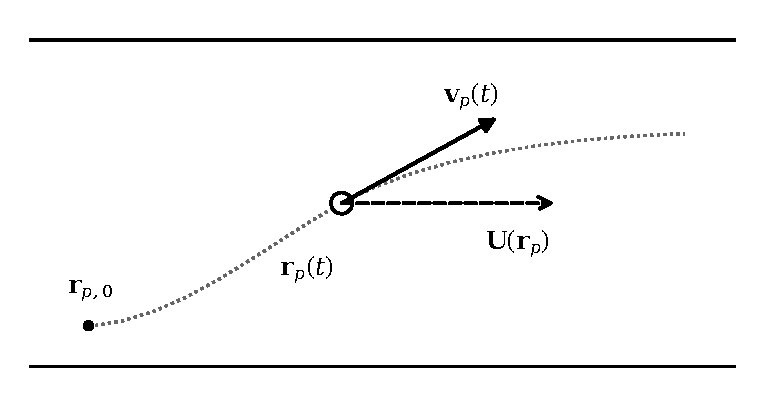
\includegraphics[width=0.68\textwidth]{figs/particle-kinematics.pdf}
\caption{نمای شماتیک مسیر ذره و بردارهای سرعت ذره و سیال.}
\label{fig:theory-particle-kinematics}
\end{figure}

مکان و سرعت ذره به‌ترتیب با $\mathbf r_p$ و $\mathbf v_p$ نمایش داده می‌شوند.
سرعت سیال در مکان لحظه‌ای ذره، $\mathbf U(\mathbf r_p)$ است.
اختلاف سرعت سیال و ذره، سرعت لغزش را تعیین می‌کند.

\begin{equation}
\mathbf w=\mathbf U(\mathbf r_p)-\mathbf v_p.
\label{eq:theory-slip-velocity}
\end{equation}

کوپل سیال و ذره در مدل‌های این پژوهش یک‌طرفه است.
میدان سیال بر ذره اثر می‌گذارد و مستقل از حرکت آن محاسبه می‌شود.
در مدل اینرسی‌دار، حرکت ذره از روابط زیر به دست می‌آید.

\begin{equation}
\begin{aligned}
\frac{\mathrm d\mathbf r_p}{\mathrm dt} &= \mathbf v_p,\\
m_{\mathrm{eff}}\frac{\mathrm d\mathbf v_p}{\mathrm dt}
&= \mathbf F_D+\mathbf F_{\mathrm{ext}} .
\end{aligned}
\label{eq:theory-particle-motion}
\end{equation}

در این روابط، $m_{\mathrm{eff}}$ جرم مؤثر و $\mathbf F_D$ نیروی درگ است.
$\mathbf F_{\mathrm{ext}}$ نیروی خارجیِ لحاظ‌شده در مدل را نشان می‌دهد.
قانون درگ و مقدار جرم مؤثر به فرض‌های هر مطالعه وابسته‌اند.

در مسئلهٔ آرایش، ذرهٔ کروی سنگین با درگ شیلر–نومان مدل می‌شود.
در بازسازی جریان، درگ استوکس و اینرسی ذره لحاظ می‌شوند.
در این دو مدل، جرم مؤثر برابر جرم ذره است.
زمان پاسخ استوکس ذره با قطر $d_p$ و چگالی $\rho_p$ محاسبه می‌شود.
\begin{equation}
\tau_p=\frac{\rho_p d_p^2}{18\mu}.
\label{eq:theory-stokes-relaxation}
\end{equation}

در مدل اینرسی‌دار مغناطیسی، جرم افزوده نیز در جرم مؤثر لحاظ می‌شود.
مدل پیش‌بینی مغناطیسی از تقریب بیش‌میرا استفاده می‌کند.
در این تقریب، موازنهٔ درگ و نیروی مغناطیسی سرعت ذره را تعیین می‌کند.

\begin{equation}
\frac{\mathrm d\mathbf r_p}{\mathrm dt}
=\mathbf U(\mathbf r_p)+\frac{\mathbf F_m}{6\pi\mu r_p}.
\label{eq:theory-overdamped-motion}
\end{equation}

در این رابطه، $\mathbf F_m$ نیروی مغناطیسی و $r_p=d_p/2$ شعاع ذره است.

\زیرقسمت{مقیاس‌های مرجع}

طول و سرعت مرجع با توجه به هندسهٔ هر مسئله انتخاب می‌شوند.
برای تشکیل آرایش، مقیاس سرعت $U_0$ برابر سرعت مرکز کانال است.
عدد رینولدز از رابطهٔ $Re=\rho_f U_0 L_0/\mu$ محاسبه می‌شود.
در این رابطه، $L_0$ طول مرجع مدل است.
اپراتور جریان از ارتفاع کانال و سرعت میانگین ورودی استفاده می‌کند.
در بازسازی، ارتفاع کانال $H$ و سرعت معلوم $U_{\mathrm{ref}}$ مقیاس‌های مرجع‌اند.
زمان مسیر با $H/U_{\mathrm{ref}}$ بی‌بعد می‌شود.
عدد استوکس از رابطهٔ $St=\tau_p U_{\mathrm{ref}}/H$ به دست می‌آید.
سرعت میانگین ورودیِ تخمینی، عدد رینولدز ورودی اپراتور را تعیین می‌کند.
در مدل مغناطیسی، شعاع لوله مقیاس مختصات عرضی است.
فاصلهٔ مشخصهٔ منبع نیز مقیاس مختصات محوری را تعیین می‌کند.

\قسمت{تشکیل آرایش چندذره‌ای با طراحی رهاسازی}
\label{sec:theory-particle-formation}

در این مسئله، موقعیت مراکز ذرات در یک زمان مشترک تعیین می‌شود.
آرایش مطلوب با انتخاب مکان، سرعت و زمان رهاسازی هر ذره شکل می‌گیرد.
پس از رهاسازی، مسیر هر ذره تحت اثر درگ جریان حامل تعیین می‌شود.

\زیرقسمت{میدان حامل و شبکهٔ فیزیک‌آگاه جریان}
\label{sec:formation-carrier-pinn}

جریان پایا در کانالی مستطیلی و دوبعدی در نظر گرفته می‌شود.
طول مرجع $L_0$ و سرعت مرکز کانال $U_0$ مبنای بی‌بعدسازی هستند.
ستاره کمیت‌های بی‌بعد را مشخص می‌کند.
برای فشار، مقدار خروجی به‌عنوان مرجع در نظر گرفته می‌شود.

\begin{equation}
\begin{aligned}
(x^*,y^*) &=
  \frac{(x^{(\mathrm{dim})},y^{(\mathrm{dim})})}{L_0},
& \mathbf U^* &= \frac{\mathbf U^{(\mathrm{dim})}}{U_0},\\
t^* &= \frac{t^{(\mathrm{dim})}U_0}{L_0},
& p^* &= \frac{p^{(\mathrm{dim})}-p_{\mathrm{out}}^{(\mathrm{dim})}}{\rho_f U_0^2},\\
(L^*,H^*,d_p^*) &=
  \frac{(L^{(\mathrm{dim})},H^{(\mathrm{dim})},d_p^{(\mathrm{dim})})}{L_0},
& \mathrm{Re} &= \frac{\rho_f U_0 L_0}{\mu}.
\end{aligned}
\label{eq:formation-nondimensionalization}
\end{equation}

سرعت ذره نیز با $U_0$ بی‌بعد می‌شود.
مقادیر بی‌بعد طول، ارتفاع و عدد رینولدز در این مطالعه عبارت‌اند از
\[
L^*=2.2,\qquad H^*=0.30,\qquad \mathrm{Re}=10.
\]
معادلات پیوستگی و مومنتوم بی‌بعد به‌صورت زیر نوشته می‌شوند.

\begin{equation}
\begin{aligned}
\nabla^*\cdot\mathbf U^* &=0,\\
(\mathbf U^*\cdot\nabla^*)\mathbf U^*
  &=-\nabla^*p^*+\frac{1}{\mathrm{Re}}\nabla^{*2}\mathbf U^*.
\end{aligned}
\label{eq:formation-flow-governing}
\end{equation}

در این روابط، $\mathbf U^*=(u^*,v^*)$ است.
مشتق‌های مکانی نسبت به $x^*$ و $y^*$ محاسبه می‌شوند.
شرط عدم لغزش روی دو دیوارهٔ افقی برقرار است.
پروفایل سرعت توسعه‌یافته در ورودی و خروجی اعمال می‌شود.
فشار بی‌بعد در خروجی صفر است.
پاسخ تحلیلی جریان پوازوی صفحه‌ای به‌صورت زیر است.

\begin{equation}
\begin{aligned}
u_{\mathrm{ref}}^*(y^*)&=
4\frac{y^*}{H^*}\left(1-\frac{y^*}{H^*}\right),\\
v_{\mathrm{ref}}^*&=0,\qquad
p_{\mathrm{ref}}^*(x^*)=
\frac{8}{\mathrm{Re}(H^*)^2}(L^*-x^*).
\end{aligned}
\label{eq:formation-poiseuille-reference}
\end{equation}

پاسخ تحلیلی درون دامنه برای ارزیابی میدان شبکه استفاده می‌شود.
آموزش شبکه از باقیماندهٔ معادلات و قیود جریان استفاده می‌کند.
مقادیر تحلیلی درون دامنه به‌عنوان برچسب آموزشی وارد نمی‌شوند.

شبکهٔ فیزیک‌آگاه هشت ورودی و سه خروجی دارد.
دو ورودی نخست، مختصات مکانی بی‌بعد هستند.
برای هر دیواره، سه ورودی مکان و مؤلفه‌های سرعت پرتاب را مشخص می‌کنند.
خروجی‌های شبکه میدان‌های $u^*$، $v^*$ و $p^*$ هستند.
شرایط مرزی با فرم زیر در خروجی شبکه اعمال می‌شوند.

\begin{equation}
\begin{aligned}
X &= \frac{x^*}{L^*},
&Y &= \frac{y^*}{H^*},
&B &= 4Y(1-Y),
&M &= X(1-X),\\
u_\theta^* &= B(1+M n_u),
&v_\theta^* &= B M n_v,
&p_\theta^* &= P_s^*(1-X)n_p,\\[-2pt]
P_s^* &= \frac{8L^*}{\mathrm{Re}(H^*)^2}.&&&&
\end{aligned}
\label{eq:formation-pinn-output}
\end{equation}

توابع $n_u$، $n_v$ و $n_p$ خروجی‌های خام شبکه هستند.
متغیرهای $X$ و $Y$ برای ساخت فرم خروجی به کار می‌روند.
تابع هزینهٔ آموزش پنج مؤلفه دارد.
دو مؤلفهٔ نخست، باقیمانده‌های پیوستگی و مومنتوم را کاهش می‌دهند.
مؤلفهٔ توسعه‌یافتگی، $v^*$ و مشتق‌های محوری سرعت را محدود می‌کند.
مؤلفهٔ دبی، شار بی‌بعد مقطع را به $2H^*/3$ نزدیک می‌کند.
مؤلفهٔ استقلال، مشتق خروجی‌ها نسبت به ورودی‌های رهاسازی را جریمه می‌کند.
در کوپل یک‌طرفه، تغییر شرایط رهاسازی میدان حامل را تغییر نمی‌دهد.
آموزش با روش آدام آغاز می‌شود و با روش \lr{L-BFGS} ادامه می‌یابد.

\زیرقسمت{معادلهٔ بی‌بعد ذره و شرایط رهاسازی}
\label{sec:formation-particle-ode}

ذرات کروی و صلب فرض می‌شوند.
قطر بی‌بعد ذره $d_p^*=0.025$ و نسبت چگالی $\beta=1000$ است.
نسبت چگالی از رابطهٔ $\beta=\rho_p/\rho_f$ به دست می‌آید.
در این مدل، درگ تنها نیروی وارد بر ذره است.
حرکت مرکز ذره از معادلات بی‌بعد زیر به دست می‌آید.

\begin{equation}
\begin{aligned}
\frac{\mathrm d\mathbf r_p^*}{\mathrm dt^*} &= \mathbf v_p^*,\\
\mathbf w^* &=
  \mathbf U^*(\mathbf r_p^*)-\mathbf v_p^*,\\
\mathrm{Re}_p &= \mathrm{Re}\,d_p^*\,\|\mathbf w^*\|,\\
\frac{\mathrm d\mathbf v_p^*}{\mathrm dt^*}
  &= \frac{18 f(\mathrm{Re}_p)}{\beta\,\mathrm{Re}\,(d_p^*)^2}\,\mathbf w^* .
\end{aligned}
\label{eq:formation-particle-ode}
\end{equation}

تابع $f$ تصحیح شیلر–نومان را در قانون درگ وارد می‌کند.
پیاده‌سازی برای عدد رینولدز ذره از رابطهٔ زیر استفاده می‌کند.

\begin{equation}
f(\mathrm{Re}_p)=
\begin{cases}
1+0.15\,\mathrm{Re}_p^{0.687}, & \mathrm{Re}_p<1000,\\
0.44\,\mathrm{Re}_p/24, & \mathrm{Re}_p\ge 1000.
\end{cases}
\label{eq:formation-drag-factor}
\end{equation}

مرکز ذره در آغاز به‌اندازهٔ شعاع و حاشیه از دیواره فاصله دارد.
حاشیهٔ بی‌بعد رهاسازی برابر $\varepsilon^*=10^{-5}$ است.
مختصات عرضی اولیه با انتخاب دیواره تعیین می‌شود.

\begin{equation}
y_{0,i}^*=
\begin{cases}
d_p^*/2+\varepsilon^*, & s_i=0,\\
H^*-d_p^*/2-\varepsilon^*, & s_i=1.
\end{cases}
\label{eq:formation-release-height}
\end{equation}

مقادیر صفر و یکِ $s_i$ به‌ترتیب دیوارهٔ پایین و بالا را مشخص می‌کنند.
در حالت آزاد، مکان محوری رهاسازی در بازهٔ $[0,L^*]$ قرار دارد.
کران‌های سرعت اولیه برای دو دیواره به‌صورت زیر هستند.

\begin{equation}
\begin{aligned}
-0.40 \le u_{0,i}^* &\le 1.50,\\
0.15 \le v_{0,i}^* &\le 1.20 && (s_i=0),\\
-1.20 \le v_{0,i}^* &\le -0.15 && (s_i=1).
\end{aligned}
\label{eq:formation-release-velocity-bounds}
\end{equation}

مؤلفهٔ عرضی سرعت اولیه در هر دو حالت به‌سمت داخل کانال است.
برای هر ذره، سه ورودی دیوارهٔ مقابل در میانهٔ بازهٔ خود ثابت‌اند.
تماس ذره با دیوارهٔ افقی، انتگرال‌گیری مسیر را متوقف می‌کند.
خروج مرکز ذره از مرزهای باز نیز انتگرال‌گیری را متوقف می‌کند.
با شرایط رهاسازی معلوم، حل معادله مسیر بی‌بعد همان ذره را می‌دهد.

\زیرقسمت{زمان‌بندی مشترک و تابع هدف آرایش}
\label{sec:formation-objective}

آرایش هدف با $N$ نقطهٔ بی‌بعد برای مراکز ذرات تعریف می‌شود.
برای ذرهٔ $i$، نقطهٔ هدف تخصیص‌یافته را $\mathbf g_i^*$ می‌نامیم.
دیواره یا ایستگاه رهاسازی یک انتخاب گسسته است.
در حالت آزاد، مکان محوری، دو سرعت اولیه و سن پرواز بهینه می‌شوند.
سن پرواز $a_i^*$ فاصلهٔ زمانی رهاسازی تا لحظهٔ تشکیل آرایش است.
زمان تشکیل و زمان رهاسازی هر ذره از روابط زیر به دست می‌آیند.

\begin{equation}
T^*=\max_i a_i^*+t_{\mathrm{lead}}^*,
\qquad
t_{\mathrm{rel},i}^*=T^*-a_i^*,
\qquad
t_{\mathrm{lead}}^*=0.25.
\label{eq:formation-common-clock}
\end{equation}

در زمان سراسری $t^*$، سن ذرهٔ $i$ برابر $t^*-t_{\mathrm{rel},i}^*$ است.
فاصلهٔ هر جفت فقط در بازهٔ حضور مشترک آن‌ها بررسی می‌شود.
این بازه از رهاسازی ذرهٔ دیرتر تا زمان $T^*$ ادامه دارد.

برای محاسبهٔ تابع هدف، سه گروه باقیمانده تعریف می‌شوند.
این گروه‌ها خطای موقعیت، پایان زودهنگام مسیر و کمبود فاصله را می‌سنجند.
$b_i^*$ سن پایان انتگرال‌گیری ذرهٔ $i$ است.
نماد $\widetilde{\mathbf r}_i^*$ مسیر ارزیابی‌شده تا آخرین سن موجود را نشان می‌دهد.
در ارزیابی نامزدها، سن درخواستی از $b_i^*$ فراتر نمی‌رود.
$a_{\max}^*$ کران بالای سن پرواز در حالت بررسی‌شده است.
$d_{ij,k}^*$ فاصلهٔ مراکز دو ذره در نمونهٔ زمانی مشترک $k$ است.
این فاصله در زمان سراسری $t_k^*$ به‌صورت زیر محاسبه می‌شود.
\[
d_{ij,k}^*=
\left\|
\widetilde{\mathbf r}_i^*(t_k^*-t_{\mathrm{rel},i}^*)-
\widetilde{\mathbf r}_j^*(t_k^*-t_{\mathrm{rel},j}^*)
\right\|.
\]
باقیمانده‌های مسئلهٔ کمترین مربعات مقید چنین‌اند.

\begin{equation}
\begin{aligned}
\mathbf e_{i,\mathrm{pos}} &=
 \frac{\widetilde{\mathbf r}_i^*(a_i^*)-\mathbf g_i^*}{H^*},\\
e_{i,\mathrm{end}} &=
 3\frac{[a_i^*-b_i^*]_+}{a_{\max}^*},\\
e_{ij,k,\mathrm{sep}} &=
 4\frac{[d_{\mathrm{search}}^*-d_{ij,k}^*]_+}{H^*}.
\end{aligned}
\label{eq:formation-optimization-residuals}
\end{equation}

نماد $[z]_+$ برابر $\max(0,z)$ است.
بهینه‌ساز مجموع مربعات این باقیمانده‌ها را کمینه می‌کند.
فاصلهٔ هدف در جست‌وجو شامل یک حاشیهٔ اضافی است.

\begin{equation}
d_{\mathrm{acc}}^*=d_p^*+0.001=0.026,
\qquad
d_{\mathrm{search}}^*=d_{\mathrm{acc}}^*+0.0003=0.0263.
\label{eq:formation-clearance-thresholds}
\end{equation}

فاصلهٔ میان ذرات با جریمهٔ کمبود فاصله کنترل می‌شود.
حرکت ذرات تحت نیروی تماس محاسبه نمی‌شود.
نامزدی که پیش از سن موردنیاز متوقف شود، پذیرفته نمی‌شود.

\زیرقسمت{حالت‌های رهاسازی و بررسی طرح نهایی}
\label{sec:formation-release-modes}

در حالت مستقل، دیواره و مکان رهاسازی برای هر ذره انتخاب می‌شوند.
سرعت اولیه و سن پرواز هر ذره نیز قابل تنظیم‌اند.
در حالت ایستگاه ثابت، سه ایستگاه روی هر دیواره قرار دارند.
مکان‌های محوری بی‌بعد آن‌ها $L^*/4$، $L^*/2$ و $3L^*/4$ هستند.

برای حروف \lr{S}، \lr{C} و \lr{T}، هر ایستگاه یک پرتاب دارد.
برای هر حرف، شش ایستگاه به شش نقطهٔ هدف تخصیص می‌یابند.
سرعت اولیه و سن پرواز برای هر ایستگاه جداگانه تعیین می‌شوند.
در آرایش متراکم اردک، حالت ایستگاه ثابت و حالت مکان آزاد بررسی می‌شوند.
هر ایستگاه ثابت می‌تواند چند ذره را در زمان‌های متفاوت رها کند.
در حالت آزاد، مکان محوری رهاسازی برای هر ذره قابل انتخاب است.
شکل~\ref{fig:formation-release-schematic} ایستگاه‌ها، نقاط هدف و ساعت مشترک را نشان می‌دهد.

\begin{figure}[htbp]
\centering
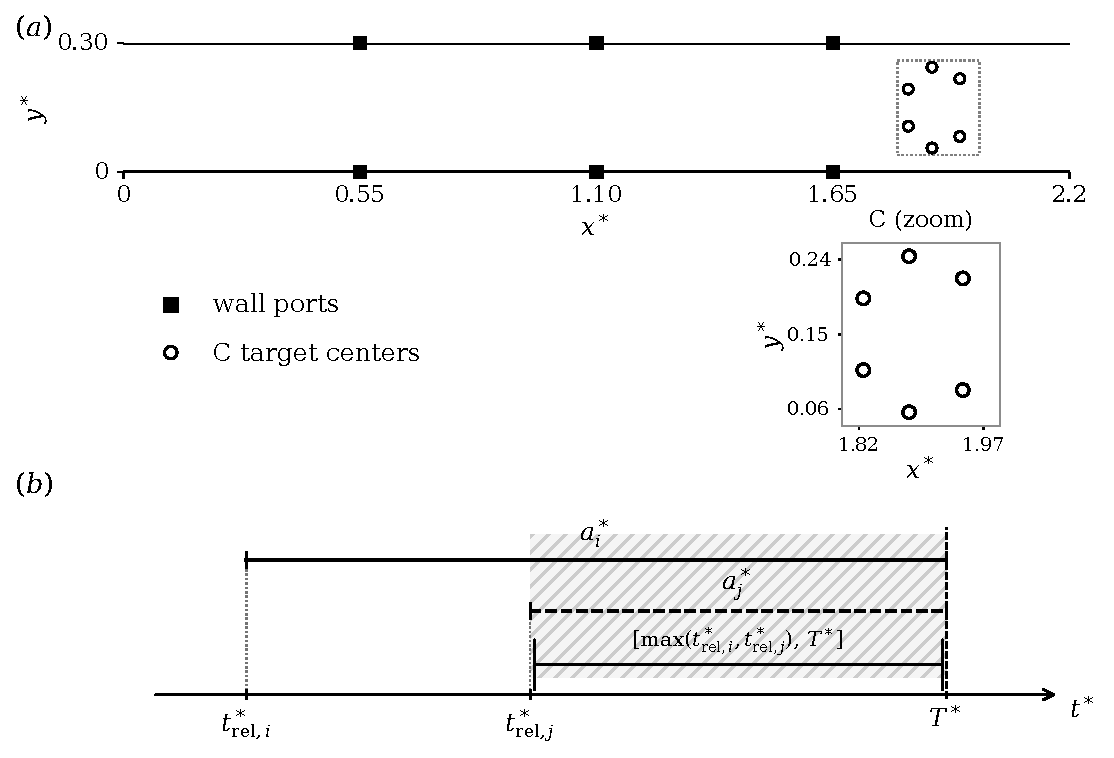
\includegraphics[width=0.93\textwidth]{figs/formation-release-schematic.pdf}
\caption{هندسهٔ بی‌بعد رهاسازی و زمان‌بندی مشترک تشکیل آرایش.}
\label{fig:formation-release-schematic}
\end{figure}

ابتدا مجموعه‌ای از مسیرهای اولیه با شرایط رهاسازی مجاز ساخته می‌شود.
سپس برای هر نقطهٔ هدف، نامزدهای مناسب رهاسازی انتخاب می‌شوند.
انتخاب‌های اولیه با توجه به خطای هدف و فاصلهٔ ذرات انجام می‌شوند.
در پالایش اولیه، میدان درون‌یابی‌شده هزینهٔ ارزیابی مسیرها را کاهش می‌دهد.
طرح‌های منتخب با ارزیابی مستقیم میدان شبکه بررسی می‌شوند.
در هر حل محلی، انتخاب‌های گسسته ثابت می‌مانند.
متغیرهای پیوسته با کمترین مربعات مقید پالایش می‌شوند.
وزن‌های شبکهٔ جریان در تمام مراحل طراحی ثابت می‌مانند.

طرح نهایی با میدان شبکه و میدان تحلیلی پوازوی بازپخش می‌شود.
هر دو بازپخش از شرایط رهاسازی و زمان‌بندی یکسان استفاده می‌کنند.
کمینهٔ فاصله با نمونه‌برداری متراکم‌تر و پالایش محلی کمینه‌ها بررسی می‌شود.
بیشینهٔ خطای موقعیت در بازپخش شبکه باید حداکثر $0.003$ باشد.
کران خطای بازپخش مرجع و اختلاف دو بازپخش $0.004$ است.
در هر دو بازپخش، کمینهٔ فاصلهٔ مراکز باید دست‌کم $0.026$ باشد.
این بررسی عددی در بازهٔ حضور مشترک هر جفت انجام می‌شود.
آرایش با مکان مراکز ذرات در لحظهٔ $T^*$ تعریف می‌شود.

\قسمت{دو مسئلهٔ مستقیم با شبکهٔ عملگر عمیق}
\label{sec:theory-forward-operators}

شبکهٔ عملگر عمیق (\lr{DeepONet})، ورودی تابعی را به تابع پاسخ نگاشت می‌کند.
این معماری دو شاخهٔ ورودی و پرس‌وجو دارد \cite{lu2021deeponet}.
شاخهٔ ورودی، نمونه‌های تابع را به ضرایب آموخته‌شده تبدیل می‌کند.
شاخهٔ پرس‌وجو، توابع پایه را در مختصات خواسته‌شده ارزیابی می‌کند.
ضرب داخلی ضرایب و پایه‌ها، پاسخ شبکه را می‌سازد.

در آموزش فیزیک‌آگاه، باقیماندهٔ معادلات در تابع هزینه وارد می‌شود \cite{wang2021pideeponet}.
در مسئلهٔ جریان، شاخهٔ پرس‌وجو مختصات مکانی را دریافت می‌کند.
در مسئلهٔ مغناطیسی، ورودی این شاخه زمان داخل پنجره است.
در هر مسئله، پروفایل سرعت یا تحریک مغناطیسی از پیش معلوم است.

\زیرقسمت{پیش‌بینی میدان جریان و مسیر ذره از پروفایل ورودی}
\label{sec:forward-flow-operator}

جریان پایا در کانال مستطیلی دوبعدی بررسی می‌شود.
ارتفاع کانال $H$ مقیاس طول است.
سرعت میانگین ورودی $\bar U$ مقیاس سرعت میدان است.
فشار نسبت به فشار مرجع خروجی بی‌بعد می‌شود.

\begin{equation}
\begin{aligned}
(x^*,y^*) &= (x/H,y/H),&
\mathbf U^* &= \mathbf U/\bar U,\\
p^* &= \frac{p-p_{\mathrm{ext}}}{\rho_f\bar U^2},&
\psi^* &= \frac{\psi}{H\bar U},\\
\mathrm{Re} &= \frac{\rho_f\bar U H}{\mu},&
\Omega^* &= (0,5)\times(0,1).
\end{aligned}
\label{eq:forward-flow-scales}
\end{equation}

در این روابط، $\psi^*$ تابع جریان بی‌بعد است.
بازهٔ آموزش عدد رینولدز از $10$ تا $100$ است.
معادلات ناویر–استوکس پایا در دامنه با همین مقیاس‌ها نوشته می‌شوند.

\begin{equation}
\begin{aligned}
\nabla^*\!\cdot\mathbf U^* &=0,\\
(\mathbf U^*\!\cdot\nabla^*)\mathbf U^*
&=-\nabla^*p^*+\mathrm{Re}^{-1}(\nabla^*)^2\mathbf U^* .
\end{aligned}
\label{eq:forward-flow-equations}
\end{equation}

پروفایل محوری ورودی $f^*(y^*)$ است.
مؤلفهٔ عرضی سرعت در ورودی صفر است.
دیواره‌ها شرط عدم لغزش دارند.
در خروجی، شرط طبیعی مطابق پیاده‌سازی به‌صورت زیر اعمال می‌شود.

\begin{equation}
\begin{aligned}
u^*(0,y^*)&=f^*(y^*), & v^*(0,y^*)&=0,\\
\mathbf U^*(x^*,0)&=\mathbf 0, &
\mathbf U^*(x^*,1)&=\mathbf 0,\\
\mathrm{Re}^{-1}\partial_{x^*}u^*(5,y^*)-p^*(5,y^*)&=0,\\
\mathrm{Re}^{-1}\partial_{x^*}v^*(5,y^*)&=0.
\end{aligned}
\label{eq:forward-flow-boundaries}
\end{equation}

\textbf{نمایش پروفایل ورودی.}
پروفایل سرعت با اسپلاین مکعبی نمایش داده می‌شود.
پروفایل ورودی در دو سر عرض کانال صفر است.
پروفایل با سرعت میانگین مثبت نرمال می‌شود.
انتگرال $f^*$ روی عرض بی‌بعد کانال برابر یک است.
پروفایل سهموی مرجع با $f_{\mathrm P}^*(y^*)=6y^*(1-y^*)$ تعریف می‌شود.
شاخهٔ ورودی اختلاف دو پروفایل را در $257$ نقطه دریافت می‌کند.
نقاط نمونه‌برداری روی کل بازهٔ عرضی یکنواخت‌اند.
دو ویژگی اسکالر نیز به این بردار اضافه می‌شوند.

\begin{equation}
\begin{aligned}
y_j^*&=j/256,\qquad j=0,\ldots,256,\\
\Delta f^*&=f^*-f_{\mathrm P}^*,\\
\boldsymbol\chi&=
\left[
\big(\Delta f^*(y_j^*)\big)_{j=0}^{256},
\frac{\log(\mathrm{Re}/10)}{\log 10},
\frac{\log(1+\kappa)}{5}
\right].
\end{aligned}
\label{eq:forward-flow-branch-input}
\end{equation}

کمیت $\kappa$ مقیاس مؤثر تغییرات پروفایل را نشان می‌دهد.
این کمیت از نسبت نرم مشتق به نرم اختلاف محاسبه می‌شود.
\[
\kappa \approx \frac{\|(\Delta f^*)'\|_2}{\pi\|\Delta f^*\|_2}.
\]
نرم‌ها روی عرض بی‌بعد کانال محاسبه می‌شوند.
در پیاده‌سازی، $\kappa$ در بازهٔ $[1,128]$ محدود می‌شود.
برای اختلاف ناچیز با پروفایل سهموی، مقدار یک به‌کار می‌رود.
انتگرال کل اسپلاین از مسیر دیگری به فرم مرزی وارد می‌شود.

\textbf{ساخت تابع جریان و فشار.}
شاخهٔ پرس‌وجو از ویژگی‌های مکانی ساخته می‌شود.
مختصات، ویژگی‌های مثلثاتی و ویژگی‌های محوری در این شاخه وارد می‌شوند.
تابع جریان و فشار هرکدام زوج شاخه‌های جداگانه دارند.
هر زوج از $64$ ضریب آموخته‌شده در ترکیب پایه‌ها استفاده می‌کند.
خروجی‌های آموخته‌شدهٔ این دو زوج را $N_\psi$ و $N_p$ می‌نامیم.

\begin{equation}
\begin{aligned}
I(y^*)&=\int_0^{y^*} f^*(\xi)\,\mathrm d\xi,\qquad
\psi_{\mathrm P}^*(y^*)=3(y^*)^2-2(y^*)^3,\\
\psi_{\mathrm{lift}}^*
&=\psi_{\mathrm P}^*+\big(I-\psi_{\mathrm P}^*\big)D_{\mathrm O}(x^*),\\
M^*&=16(y^*)^2(1-y^*)^2(1-e^{-x^*/0.1})^2,\\
\psi^*&=\psi_{\mathrm{lift}}^*+M^*N_\psi,\\
p^*&=\frac{12(5-x^*)}{\mathrm{Re}}+p_{\mathrm O}^*+N_p.
\end{aligned}
\label{eq:forward-flow-lift}
\end{equation}

در این روابط، $D_{\mathrm O}$ عامل کاهش اثر ورودی در راستای محور است.
عامل کاهش و تصحیح فشار از تقریب خطی‌شدهٔ اوسین به دست می‌آیند.

\begin{equation}
\begin{aligned}
k&=\pi\kappa,\qquad
\lambda=\frac{2k^2}{\sqrt{\mathrm{Re}^2+4k^2}+\mathrm{Re}},\\
\delta&=\frac{\mathrm{Re}\lambda}{k+\lambda},\\
D_{\mathrm O}(x^*)&=e^{-\lambda x^*}
\left(1-\lambda\frac{e^{-\delta x^*}-1}{\delta}\right),\\
p_{\mathrm O}^*(x^*,y^*)&=
\frac{k+\lambda}{\mathrm{Re}}\Delta f^*(y^*)e^{-kx^*}.
\end{aligned}
\label{eq:forward-flow-oseen}
\end{equation}

انتگرال $I$ در فرم مرزی تمام گره‌های اسپلاین را حفظ می‌کند.
فرم تابع جریان، شرایط سرعت ورودی و دیواره‌ها را برقرار می‌کند.
سرعت از مشتق‌های تابع جریان به دست می‌آید.
\[
u^*=\partial_{y^*}\psi^*,\qquad
v^*=-\partial_{x^*}\psi^*.
\]
این تعریف، معادلهٔ پیوستگی را در ساختار خروجی برقرار می‌کند.
شکل~\ref{fig:forward-flow-operator} دو مسیر ورود اسپلاین را نشان می‌دهد.

\begin{figure}[htbp]
\centering
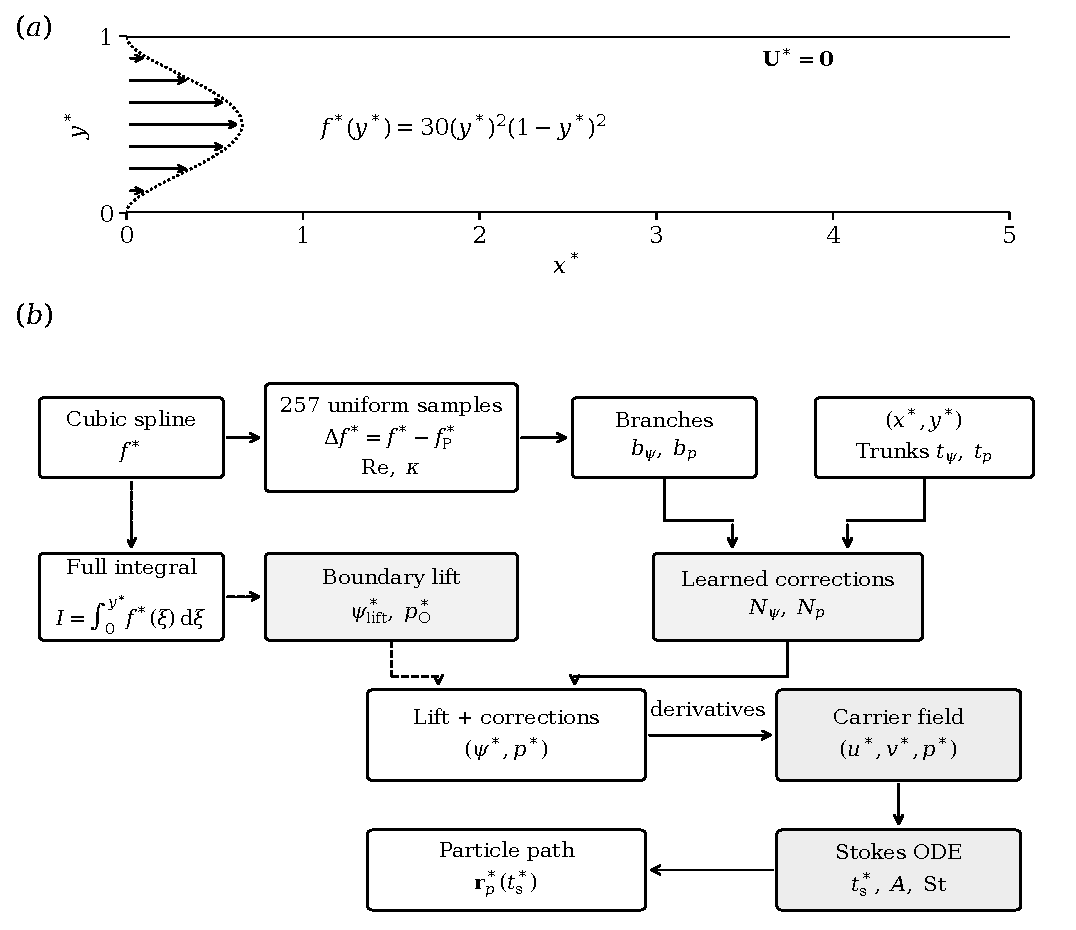
\includegraphics[width=0.93\textwidth]{figs/deeponet-flow-forward.pdf}
\caption{دامنهٔ بی‌بعد و نگاشت پروفایل ورودی به میدان و مسیر ذره.}
\label{fig:forward-flow-operator}
\end{figure}

\textbf{آموزش و محاسبهٔ مسیر.}
تابع هزینه شامل باقیماندهٔ مومنتوم غیرخطی و شرط طبیعی خروجی است.
در پیکربندی منتخب، سهم مومنتوم برحسب انحنای پروفایل ورودی مقیاس‌بندی می‌شود.
اگر $\mathbf R_{\mathrm{NS}}^*$ و $\mathbf R_{\mathrm{out}}^*$ دو باقیمانده باشند، هزینه چنین است.
\begin{equation}
\mathcal L_{\mathrm f}=
\left\langle
\frac{\|\mathbf R_{\mathrm{NS}}^*\|^2}
 {1+\|(f^*)''\|_2/\mathrm{Re}}
\right\rangle_{\Omega^*}
+10\left\langle\|\mathbf R_{\mathrm{out}}^*\|^2\right\rangle_{\mathrm{out}}.
\label{eq:forward-flow-training-loss}
\end{equation}
میانگین‌ها روی نقاط هم‌مکانی و نمونه‌های ورودی گرفته می‌شوند.
حل اجزای محدود فقط برای ارزیابی میدان استفاده می‌شود.

برای محاسبهٔ مسیر، سرعت سیال در مکان لحظه‌ای ذره خوانده می‌شود.
در این مطالعه، اینرسی ذره و درگ استوکس لحاظ می‌شوند.
زمان مسیر با سرعت مرجع معلوم $U_{\mathrm{ref}}$ بی‌بعد می‌شود.
نسبت مقیاس‌های سرعت را با $A=\bar U/U_{\mathrm{ref}}$ نشان می‌دهیم.

\begin{equation}
\begin{aligned}
t_{\mathrm s}^*&=t U_{\mathrm{ref}}/H,\qquad
\mathrm{St}=\tau_p U_{\mathrm{ref}}/H,\\
\frac{\mathrm d\mathbf r_p^*}{\mathrm dt_{\mathrm s}^*}
&=\mathbf v_{p,\mathrm s}^*,\\
\frac{\mathrm d\mathbf v_{p,\mathrm s}^*}{\mathrm dt_{\mathrm s}^*}
&=\frac{A\mathbf U^*(\mathbf r_p^*)-\mathbf v_{p,\mathrm s}^*}{\mathrm{St}}.
\end{aligned}
\label{eq:forward-flow-stokes-path}
\end{equation}

سرعت $\mathbf v_{p,\mathrm s}^*$ با $U_{\mathrm{ref}}$ مقیاس می‌شود.
انتگرال‌گیری با مکان و سرعت اولیهٔ معلوم انجام می‌شود.
در مسئلهٔ معکوس، همین زنجیره مسیر را برای ورودی‌های نامزد محاسبه می‌کند.
وزن‌های گام $94000$ مبنای بازسازی معکوس هستند.
این وزن‌ها همهٔ معیارهای پذیرش عمومی میدان را برآورده نکردند.
خطاهای میدان و باقیماندهٔ معادلات در فصل نتایج گزارش می‌شوند.

\زیرقسمت{پیش‌بینی مسیر ذره از دو تحریک مغناطیسی}
\label{sec:forward-magnetic-operator}

حرکت ذره در صفحهٔ محوری‌ـ‌عرضی یک لولهٔ دایره‌ای مستقیم بررسی می‌شود.
جریان حامل، پروفایل پوازوی کاملاً توسعه‌یافته دارد.
دو منبع ثابت در دو سوی لوله قرار دارند.
دامنهٔ هر منبع با تابعی بی‌بعد و زمان‌متغیر تعیین می‌شود.

\textbf{مقیاس‌ها و میدان دو منبع.}
شعاع لوله $R$ و فاصلهٔ مشخصهٔ منبع $D$ مقیاس‌های مکانی هستند.
سرعت مرجع محوری برابر دو برابر سرعت میانگین مرجع است.
میدان مغناطیسی با مقیاس ثابت $B_s$ بی‌بعد می‌شود.
برای منبع ایده‌آل، $M_s$ مغناطش و $R_m$ شعاع مشخصهٔ منبع است.
\[
B_s=\frac{\mu_0 M_s}{2}\left(\frac{R_m}{D}\right)^2,
\qquad R_m/D=1/2.
\]

\begin{equation}
\begin{aligned}
X&=x/R,& Z&=z/D,& \xi&=x/D=\epsilon X,\\
\epsilon&=R/D=0.001875,&
\tau&=\frac{2U_{\mathrm{ref}}t}{D},&
\mathbf q&=(X,Z),\\
\mathbf B^*&=\mathbf B/B_s,&
\bar U^*&=\bar U/U_{\mathrm{ref}}.
\end{aligned}
\label{eq:forward-mag-scales}
\end{equation}

سرعت مرجع $U_{\mathrm{ref}}$ در این زیربخش به مدل مغناطیسی تعلق دارد.
نسبت شعاع ذره به شعاع لوله $r_p/R=1/150$ است.
در معادلهٔ میدان، مشتق‌گیری نسبت به $(\xi,Z)$ انجام می‌شود.
برای منبع چپ و راست، $\sigma$ به‌ترتیب $+1$ و $-1$ است.

\begin{equation}
\begin{aligned}
Y_\sigma&=1+\sigma\xi,\qquad
S_\sigma=Y_\sigma^2+Z^2,\\
\mathbf b_\sigma(\xi,Z)&=
\frac{1}{S_\sigma^2}
\begin{pmatrix}
\sigma(Y_\sigma^2-Z^2)\\[2pt] 2Y_\sigma Z
\end{pmatrix},\\
\mathbf B^*(\xi,Z,\tau)&=
 a_L(\tau)\mathbf b_{+1}(\xi,Z)+a_R(\tau)\mathbf b_{-1}(\xi,Z).
\end{aligned}
\label{eq:forward-mag-field}
\end{equation}

توابع $\mathbf b_\sigma$ شکل فضایی ثابت هر منبع را مشخص می‌کنند.
توابع $a_L$ و $a_R$ دامنه‌های علامت‌دار منابع هستند.
قید تحریک در هر زمان $|a_L|+|a_R|\le\sqrt{0.5}$ است.

\textbf{نیروی مغناطیسی و معادلهٔ حرکت.}
مغناطش القایی ذره خطی و بدون اشباع فرض می‌شود.
ضریب قطبش ذره برابر $\alpha=3V_p/\mu_0$ است.
در این تعریف، $V_p$ حجم ذره و $\mu_0$ تراوایی خلأ است.
مقیاس نیرو برابر $F_s=\alpha B_s^2/D$ انتخاب می‌شود.
با این مقیاس، نیروی بی‌بعد به‌صورت زیر نوشته می‌شود.

\begin{equation}
\begin{aligned}
\mathbf F_m^*&=\frac{\mathbf F_m}{F_s}
=\frac12\nabla_{(\xi,Z)}\|\mathbf B^*\|^2\\
&=\frac{a_L^2}{2}\nabla_{(\xi,Z)}\|\mathbf b_{+1}\|^2
 +\frac{a_R^2}{2}\nabla_{(\xi,Z)}\|\mathbf b_{-1}\|^2\\
&\quad+a_La_R\nabla_{(\xi,Z)}
 \big(\mathbf b_{+1}\!\cdot\mathbf b_{-1}\big).
\end{aligned}
\label{eq:forward-mag-force}
\end{equation}

جملهٔ آخر اثر هم‌زمانی دو منبع را در نیرو وارد می‌کند.
در تقریب بیش‌میرا، درگ استوکس و نیروی مغناطیسی موازنه می‌شوند.
معادلهٔ بی‌بعد حرکت در مختصات محوری‌ـ‌عرضی چنین است.

\begin{equation}
\begin{aligned}
\frac{\mathrm d\mathbf q}{\mathrm d\tau}
&=\begin{pmatrix}0\\\bar U^*(1-X^2)\end{pmatrix}
+\Gamma
  \begin{pmatrix}1&0\\0&\epsilon\end{pmatrix}
  \mathbf F_m^*(\epsilon X,Z,\tau)
=:\mathbf G(\mathbf q,\mathbf a;\boldsymbol\pi),\\
\Gamma&=\frac{\alpha B_s^2}{12\pi\mu r_p U_{\mathrm{ref}}R},
\qquad \mathbf a=(a_L,a_R).
\end{aligned}
\label{eq:forward-mag-motion}
\end{equation}

در این معادله، $\boldsymbol\pi$ مجموعهٔ پارامترهای سیال را مشخص می‌کند.
گرانروی مرجع $\mu_{\mathrm{ref}}$ همان مقیاس نرمال‌سازی شاخهٔ ورودی است.
در نمونه‌های آموزش، سرعت و گرانروی بی‌بعد در بازه‌های زیر قرار دارند.
\[
1/3\le\bar U^*\le2,\qquad
20/49\le \mu/\mu_{\mathrm{ref}}\le120/49.
\]
ضریب $\Gamma$ و عامل $\epsilon$ هر دو بی‌بعد هستند.
عامل $\epsilon$ تفاوت مقیاس محوری و عرضی را لحاظ می‌کند.
زمان آرامش با مقیاس زمانی $D/(2U_{\mathrm{ref}})$ بی‌بعد می‌شود.
برای برآورد آن، جرم مؤثر شامل نصف جرم سیال جابه‌جاشده است.
\[
\tau_p^*=
\frac{2U_{\mathrm{ref}}}{D}
\frac{2(\rho_p+\rho_f/2)r_p^2}{9\mu}.
\]
زمان آرامش بی‌بعد در بازهٔ پارامترها حدود $4\times10^{-8}$ تا $2.4\times10^{-7}$ است.
این زمان از کوتاه‌ترین پنجرهٔ آموزش بسیار کوچک‌تر است.
تقریب بیش‌میرا برای تحریک‌هایی با تغییرات کندتر از آرامش ذره به‌کار می‌رود.
گرانش، حرکت براونی و تصحیح درگ نزدیک دیواره در مدل حذف شده‌اند.

\textbf{عملگر پنجره‌ای مسیر.}
در هر پنجره، زمان پرس‌وجو با $s=(\tau-\tau_j)/h$ تعریف می‌شود.
طول بی‌بعد پنجره $h$ و مکان آغازین آن $\mathbf q_j$ است.
هر منبع در $17$ زمان یکنواخت نمونه‌برداری می‌شود.
دامنهٔ تحریک میان نمونه‌ها با درون‌یابی خطی محاسبه می‌شود.
نمونه‌های دو منبع، مکان آغازین و طول پنجره وارد شاخهٔ ورودی می‌شوند.
نمایش نرمال‌شدهٔ گرانروی، سرعت میانگین و چگالی نیز وارد همین شاخه می‌شود.
در معادلهٔ بیش‌میرا، چگالی مستقیماً وارد سرعت ذره نمی‌شود.
شاخهٔ پرس‌وجو زمان نرمال‌شدهٔ $s$ را دریافت می‌کند.
تصحیح هر مؤلفه از ضرب داخلی دو بردار $48$مؤلفه‌ای ساخته می‌شود.

\begin{equation}
\begin{aligned}
\mathbf q_\theta(s)&=
\mathbf q_j+
h\int_0^s \mathbf G\big(\mathbf q_j,\mathbf a(\zeta);\boldsymbol\pi\big)\,\mathrm d\zeta
+h^2s^2E_a\,\mathbf C_\theta(s),\\
E_a&=\frac{1}{17\,a_{\max}^2}
\sum_{k=0}^{16}(a_{L,k}^2+a_{R,k}^2),
\qquad a_{\max}=\sqrt{0.5}.
\end{aligned}
\label{eq:forward-mag-window}
\end{equation}

در انتگرال، $\mathbf a(\zeta)$ تحریک درون‌یابی‌شده در زمان محلی است.
جملهٔ انتگرالی، میدان و جریان را در مکان آغاز پنجره ارزیابی می‌کند.
انتگرال زمانی برای نمایش خطی تحریک به‌صورت تحلیلی محاسبه می‌شود.
تصحیح $\mathbf C_\theta$ از ترکیب خروجی دو شاخه به دست می‌آید.
عامل $s^2$ شرط اولیهٔ مکان را دقیق برقرار می‌کند.
عامل $E_a$ تصحیح را برای تحریک صفر حذف می‌کند.
شرط اولیهٔ مدل بیش‌میرا فقط مکان آغازین را مشخص می‌کند.

\textbf{آموزش و اتصال پنجره‌ها.}
تابع هزینه از میانگین مربعات باقیماندهٔ بی‌بعد حرکت ساخته می‌شود.
در پیاده‌سازی، باقیمانده با طول پنجره نیز مقیاس‌بندی می‌شود.

\begin{equation}
\mathbf R_{\mathrm m}(s)=
\frac{h^{-1}\partial_s\mathbf q_\theta
-\mathbf G(\mathbf q_\theta,\mathbf a(s);\boldsymbol\pi)}{h},
\qquad
\mathcal L_{\mathrm m}=\left\langle\|\mathbf R_{\mathrm m}\|^2/2\right\rangle .
\label{eq:forward-mag-training-loss}
\end{equation}

مسیرهای حاصل از حل مستقل در آموزش وارد نمی‌شوند.
آموزش پنجره‌های بی‌بعد $0.00625\le h\le0.10$ را پوشش می‌دهد.
پیش‌بینی پیوسته با انتقال مکان نهایی هر پنجره به پنجرهٔ بعد انجام می‌شود.
طول پیش‌فرض پنجرهٔ پیش‌بینی $0.05$ است.
نگاشت‌های محلی بلندتر از $0.05$ به دو نیم‌پنجره تقسیم می‌شوند.
بازهٔ مکانی ارزیابی $|X|\le0.7$ و $-2\le Z\le1.7$ است.
تعمیم به دامنهٔ تحریک و وضوح نمونه‌برداری هر پنجره وابسته است.
حل عددی مستقل معادلهٔ حرکت، مرجع مقایسهٔ مسیر است.
شکل~\ref{fig:forward-magnetic-operator} تحریک، هندسه و اتصال پنجره‌ها را نشان می‌دهد.

\begin{figure}[htbp]
\centering
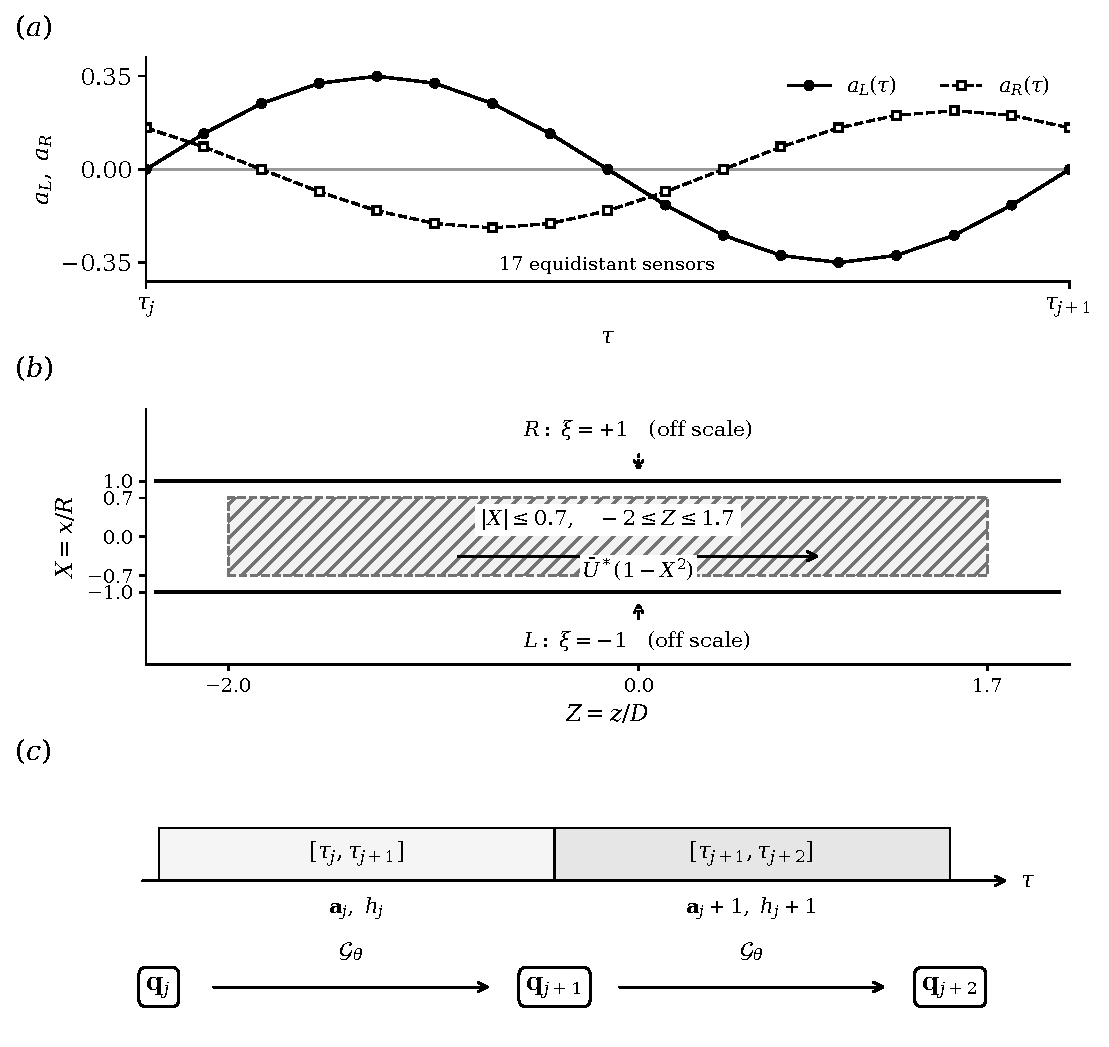
\includegraphics[width=0.93\textwidth]{figs/deeponet-magnetic-forward.pdf}
\caption{تحریک دو منبع، نمای محوری‌ـ‌عرضی لوله و اتصال پنجره‌های بی‌بعد.}
\label{fig:forward-magnetic-operator}
\end{figure}

\قسمت{دو مسئلهٔ معکوس از روی حرکت ذره}
\label{sec:theory-inverse-problems}

در مسئلهٔ معکوس، حرکت ذره برای تخمین ورودی مدل استفاده می‌شود.
در مسئلهٔ جریان، ورودی کانال از دو مسیر ذره تخمین زده می‌شود.
در مسئلهٔ مغناطیسی، مسیر برای تعیین تحریک منابع به کار می‌رود.
مقیاس‌های بی‌بعد هر مسئله از صورت‌بندی مستقیم آن گرفته می‌شوند.

\زیرقسمت{بازسازی جریان از دو مسیر زمان‌دار}
\label{sec:inverse-flow-timed}

\textbf{داده‌ها و مجهول‌ها.}
در کانال مستطیلی بی‌بعد $5\times1$، تعداد $N_p$ مسیر زمان‌دار داده می‌شود.
مکان و بردار سرعت اولیهٔ هر ذره معلوم‌اند.
زمان پاسخ استوکس هر ذره و گرانروی سیال نیز معلوم‌اند.
در این بخش، $t^*$ همان زمان بی‌بعد مسیر در بخش قبل است.
عدد استوکس ذرهٔ $i$ با $\mathrm{St}_i=\tau_{p,i}U_{\mathrm{ref}}/H$ تعریف می‌شود.
زمان هر مسیر از نخستین مشاهدهٔ آن شروع می‌شود.

مجهول‌ها شکل پروفایل ورودی و سرعت میانگین آن هستند.
اسپلاین مکعبی پروفایل با مقادیر گره‌ای پارامترگذاری می‌شود.
پروفایل سهموی $f_{\mathrm P}^*(y^*)=6y^*(1-y^*)$ شکل پایه است.
مقادیر گره‌ای از ضرب شکل پایه در ضرایب مثبت ساخته می‌شوند.
یک ضریب لگاریتمی داخلی برای حذف ابهام نرمال‌سازی ثابت می‌شود.

\begin{equation}
\begin{aligned}
\widetilde f(y_j^*)&= f_{\mathrm P}^*(y_j^*)\,e^{c_j},\\
f^*(y^*)&=\frac{\widetilde f(y^*)}{\int_0^1\widetilde f(s)\,\mathrm ds},
& A&=\bar U/U_{\mathrm{ref}},\\
\mathrm{Re}_{\mathrm{ref}}&=\frac{\rho_f U_{\mathrm{ref}}H}{\mu},
& \mathrm{Re}&=A\,\mathrm{Re}_{\mathrm{ref}} .
\end{aligned}
\label{eq:inverse-flow-parameterization}
\end{equation}

مقادیر گره‌ای دو انتهای عرض کانال صفر هستند.
کران سرعت میانگین، عدد رینولدز را در دامنهٔ آموزش نگه می‌دارد.
در طول برازش، وزن‌های اپراتور جریان ثابت می‌مانند.
اپراتور با $f^*$ و $\mathrm{Re}$، سرعت و فشار را برمی‌گرداند.
در مقیاس مرجع مسیر، خروجی‌های سرعت و فشار به‌ترتیب چنین‌اند.

\[
\mathbf U_{\mathrm{ref}}^*=A\mathbf U_\theta^*,
\qquad
p_{\mathrm{ref}}^*=A^2p_\theta^*.
\]

فشار از پاسخ اپراتور استنباط می‌شود.

\textbf{برازش انتگرالی مسیر.}
مدل ذره همان معادلهٔ استوکس بخش~\ref{sec:forward-flow-operator} است.
با انتگرال‌گیری از رابطهٔ~\eqref{eq:forward-flow-stokes-path}، رابطهٔ زیر برای مکان به دست می‌آید.
در برازش، میدان روی درون‌یابی خطی موقعیت‌های مشاهده‌شده ارزیابی می‌شود.

\begin{equation}
\begin{aligned}
\widehat{\mathbf r}_{i,\mathrm{int}}^*(t^*)
&=\mathbf r_{i,0}^*
 +\mathrm{St}_i(1-e^{-t^*/\mathrm{St}_i})\,\mathbf v_{i,0}^*\\
&\quad+\int_0^{t^*}
  (1-e^{-(t^*-\xi)/\mathrm{St}_i})\,
  A\mathbf U_\theta^*(\mathbf r_{i,\mathrm{obs}}^*(\xi))\,\mathrm d\xi .
\end{aligned}
\label{eq:inverse-flow-integral-path}
\end{equation}

در این رابطه، سرعت اولیه با $U_{\mathrm{ref}}$ بی‌بعد شده است.
انتگرال هر فاصلهٔ زمانی با قاعدهٔ گاوس محاسبه می‌شود.
این فرم نیاز به مشتق‌گیری مرتبهٔ دوم از دادهٔ موقعیت را برطرف می‌کند.
خطای موقعیت برای هر مسیر با تعداد نمونه‌های آن نرمال می‌شود.

\begin{equation}
\begin{aligned}
\mathcal J_{\mathrm{path}}
&=\frac{1}{N_p}\sum_{i=1}^{N_p}\frac{1}{n_i}
\sum_{k=1}^{n_i}
\left\|
\frac{\widehat{\mathbf r}_{i,\mathrm{int}}^*(t_{i,k}^*)
-\mathbf r_{i,\mathrm{obs}}^*(t_{i,k}^*)}{\sigma_x^*}
\right\|^2,\\
\mathcal J_{\mathrm{timed}}
&=\mathcal J_{\mathrm{path}}
+\mathcal J_{\mathrm{prior}}+\mathcal J_{\mathrm{mom}}+\mathcal J_+.
\end{aligned}
\label{eq:inverse-flow-timed-objective}
\end{equation}

در مثال‌های پایه، $N_p=2$ است.
در بررسی تعداد ذرات، $N_p$ از دو تا شش تغییر می‌کند.
میانگین‌گیری روی ذرات، مقیاس نسبی جملهٔ منظم‌سازی را ثابت نگه می‌دارد.

$n_i$ تعداد نمونه‌های پس از مشاهدهٔ آغازین است.
$\sigma_x^*$ مقیاس بی‌بعد خطای موقعیت است.
پیشین پروفایل، همواری و انحراف از شکل سهموی را کنترل می‌کند.
پیشین سرعت، مقدار $\log A$ را به صفر نزدیک می‌کند.
در تنظیم انحنای ورودی، اجزای پیشین به‌صورت زیر هستند.

\begin{equation}
\begin{aligned}
\mathcal J_{\mathrm{prior}} &=
\lambda_c\int_0^1[(f^*)''(y^*)]^2\,\mathrm dy^*
 +\lambda_f\langle c_j^2\rangle+\lambda_A(\log A)^2,\\
\mathcal J_{\mathrm{mom}} &=
\lambda_m\left\langle
\left\|\frac{A^2\mathbf R_{\mathrm{NS}}^*}{\sigma_m^*}\right\|^2
\right\rangle_{\Omega^*}.
\end{aligned}
\label{eq:inverse-flow-prior-physics}
\end{equation}

باقیماندهٔ مومنتوم روی نقاطی مستقل از مسیرها ارزیابی می‌شود.
$\mathcal J_+$ بخش‌های منفی اسپلاین را روی شبکه‌ای متراکم جریمه می‌کند.
پس از برازش، کمینهٔ خود اسپلاین نیز بررسی می‌شود.
بهینه‌سازی مقید با روش \lr{L-BFGS-B} و چند مقدار اولیه انجام می‌شود.
از میان نامزدهای مجاز، پاسخ با کمترین هزینه انتخاب می‌شود.

\textbf{بازپخش مستقل و معیارهای ارزیابی.}
در بازپخش، معادلهٔ حرکت از شرایط اولیهٔ معلوم انتگرال‌گیری می‌شود.
میدان این بار در مکان لحظه‌ای ذرهٔ محاسبه‌شده خوانده می‌شود.
شکل~\ref{fig:inverse-flow-fit-replay} تفاوت مکان ارزیابی میدان را در دو مرحله نشان می‌دهد.

\begin{figure}[htbp]
\centering
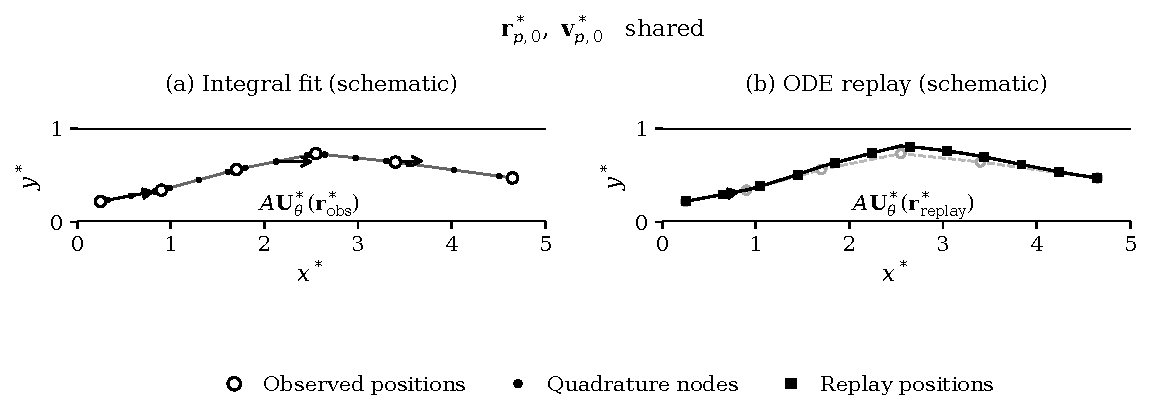
\includegraphics[width=0.93\textwidth]{figs/inverse-flow-fit-replay.pdf}
\caption{برازش روی مسیر مشاهده‌شده و بازپخش در میدان تخمینی.}
\label{fig:inverse-flow-fit-replay}
\end{figure}

دو مسیر تنها بخش‌هایی از دامنهٔ جریان را نمونه‌برداری می‌کنند.
مسیرهای مشابه می‌توانند با پروفایل‌ها و میدان‌های متفاوت سازگار باشند.
در فصل نتایج، خطای مسیر، پروفایل ورودی و میدان جداگانه گزارش می‌شوند.

\زیرقسمت{بازسازی جریان از هندسهٔ دو مسیر بدون زمان اندازه‌گیری‌شده}
\label{sec:inverse-flow-geometry}

\textbf{دادهٔ هندسی و زمان‌بندی پنهان.}
دادهٔ مسیر شامل موقعیت‌های مرتب‌شدهٔ ذره روی منحنی است.
مکان و بردار سرعت اولیهٔ غیرصفر همچنان معلوم فرض می‌شوند.
زمان پاسخ استوکس هر ذره نیز معلوم است.
مشاهدات هر منحنی برحسب طول قوس بی‌بعد یکنواخت بازنمونه‌برداری می‌شوند.
تراکم نمونه‌های اولیه به‌عنوان دادهٔ زمان وارد برازش نمی‌شود.

برای هر مسیر، زمان بی‌بعد تابعی صعودی از طول قوس است.
طول قوس با ارتفاع کانال $H$ بی‌بعد می‌شود.
اسپلاین مکعبی، تغییر نرخ زمان نسبت به طول قوس را نمایش می‌دهد.
گره آغازین اسپلاین صفر است.
مقدار نرخ آغازین از اندازهٔ سرعت اولیه تعیین می‌شود.

\begin{equation}
\begin{aligned}
\eta_i&=s^*/L_i^*,\qquad b_i(0)=0,\qquad t_i^*(0)=0,\\
\frac{\mathrm dt_i^*}{\mathrm ds^*}
&=\frac{\exp\!\left[b_{\max}\tanh\!\left(b_i(\eta_i)/b_{\max}\right)\right]}
{\|\mathbf v_{i,0}^*\|}>0 .
\end{aligned}
\label{eq:inverse-flow-positive-clock}
\end{equation}

$L_i^*$ طول قوس بی‌بعد منحنی و $b_i$ اسپلاین پنهان آن است.
زمان هر نقطه با انتگرال‌گیری ذوزنقه‌ای از نرخ مثبت محاسبه می‌شود.
شکل~\ref{fig:inverse-flow-geometry-clock} پیوند نمونه‌های هندسی و زمان‌بندی را نشان می‌دهد.

\begin{figure}[htbp]
\centering
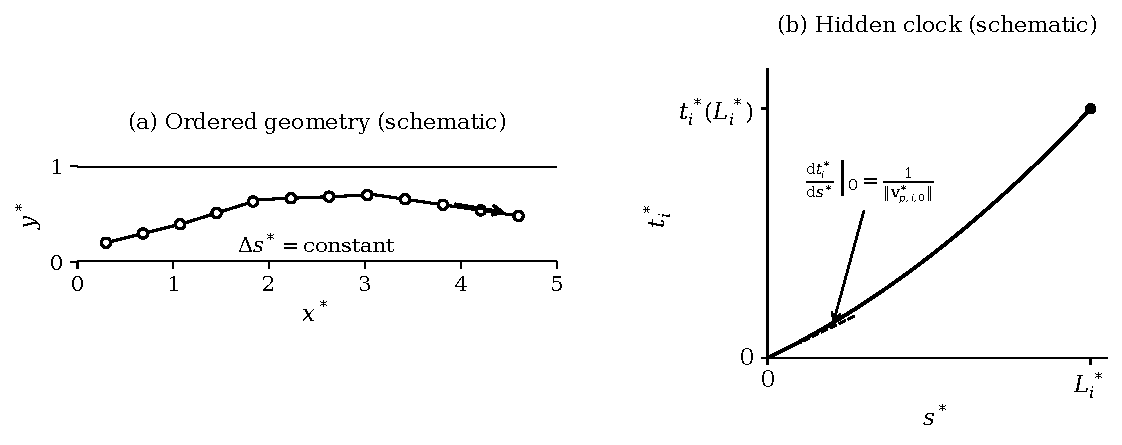
\includegraphics[width=0.9\textwidth]{figs/inverse-geometry-clock.pdf}
\caption{بازنمونه‌برداری برحسب طول قوس و زمان‌بندی صعودی مسیر.}
\label{fig:inverse-flow-geometry-clock}
\end{figure}

\textbf{برازش مشترک و ارزیابی هندسی.}
پروفایل، سرعت میانگین و دو زمان‌بندی به‌طور هم‌زمان تخمین زده می‌شوند.
زمان‌های تخمینی در رابطهٔ انتگرالی~\eqref{eq:inverse-flow-integral-path} جای‌گذاری می‌شوند.
وزن‌های اپراتور جریان در این حالت نیز ثابت می‌مانند.
به هزینهٔ مشترک، جریمهٔ اختلاف مرتبهٔ دوم گره‌های زمان‌بندی افزوده می‌شود.

\begin{equation}
\begin{aligned}
\mathcal J_{\mathrm{geo}}
&=\mathcal J_{\mathrm{path,geo}}+\mathcal J_{\mathrm{prior}}
+\mathcal J_{\mathrm{mom}}+\mathcal J_+\\
&\quad+\lambda_t\left\langle
(\Delta^2 b_{i,j})^2
\right\rangle_{i,j}.
\end{aligned}
\label{eq:inverse-flow-geometry-objective}
\end{equation}

در $\mathcal J_{\mathrm{path,geo}}$، خطا روی نقاط بازنمونه‌برداری‌شده محاسبه می‌شود.
مدت تخمینی مسیر، افق بازپخش مستقل را تعیین می‌کند.
ارزیابی از فاصلهٔ هندسی دو منحنی و تناظر طول قوس استفاده می‌کند.
$\mathcal P$ و $\mathcal Q$ به‌ترتیب منحنی مشاهده‌شده و بازپخش‌شده‌اند.
نمونه‌های هر منحنی روی طول قوس نرمال‌شدهٔ خودش یکنواخت‌اند.
فاصلهٔ $d(\mathbf p,\mathcal Q)$ کمینهٔ فاصله تا پاره‌خط‌های $\mathcal Q$ است.

\begin{equation}
\begin{aligned}
E_{\mathrm{sym}}^*
&=\left[
\tfrac12\left(
\langle d(\mathbf p_j,\mathcal Q)^2\rangle_j
+\langle d(\mathbf q_j,\mathcal P)^2\rangle_j
\right)\right]^{1/2},\\
E_{\mathrm{arc}}^*
&=\left[\langle\|\mathbf p_j-\mathbf q_j\|^2\rangle_j\right]^{1/2}.
\end{aligned}
\label{eq:inverse-flow-geometry-errors}
\end{equation}

معیار دوم ترتیب حرکت را با مقایسهٔ طول قوس نسبی لحاظ می‌کند.
دو اجرای موجود در تنظیمات و بودجهٔ بهینه‌سازی نیز تفاوت دارند.
این تفاوت‌ها در تفسیر مقایسهٔ فصل نتایج لحاظ می‌شوند.

\زیرقسمت{تخمین تحریک مغناطیسی از حرکت ذره}
\label{sec:inverse-magnetic-drive}

\textbf{رهگیری مسیر هدف در مدل نهم.}
روش موجود، مسیر هدف $X_{\mathrm{tar}}(Z)$ را دریافت می‌کند.
مختصات $X$، $Z$ و زمان $\tau$ مطابق بخش مغناطیسی بی‌بعد می‌شوند.
مدل اینرسی‌دار، حالت بعدی را از مکان و سرعت فعلی پیش‌بینی می‌کند.
سرعت بی‌بعد $\mathbf V$ مشتق مکان $\mathbf q$ نسبت به $\tau$ است.
تحریک مؤثر $c$ یک متغیر اسکالر و محدود است.
علامت تحریک، منبع فعال و قدرمطلق آن اندازهٔ اثر را تعیین می‌کند.
در هر گام، تحریک طی یک پنجرهٔ بی‌بعد ثابت نگه داشته می‌شود.

\begin{equation}
\begin{aligned}
(\mathbf q_{k+1}(c),\mathbf V_{k+1}(c))
&=\mathcal T_9(\mathbf q_k,\mathbf V_k,c;h_9),\\
e_k(c)&=X_{k+1}(c)-X_{\mathrm{tar}}(Z_{k+1}(c)),\\
h_9&=0.025,\qquad -0.5\le c\le0.5 .
\end{aligned}
\label{eq:inverse-master9-tracking}
\end{equation}

اگر خطای دو انتهای بازه علامت مخالف داشته باشد، ریشه جست‌وجو می‌شود.
اگر یکی از خطاها صفر باشد، همان انتها ریشه است.
در غیر این صورت، سه تحریک $-0.5$، $0$ و $0.5$ مقایسه می‌شوند.
تحریک منتخب در این حالت کمترین قدرمطلق خطا را دارد.
تحریک‌های انتخاب‌شده با حل‌گر مستقل اینرسی‌دار \lr{Radau} بازپخش می‌شوند.
شکل~\ref{fig:inverse-magnetic-master9} روند انتخاب تحریک و به‌روزرسانی حالت را نشان می‌دهد.

\begin{figure}[htbp]
\centering
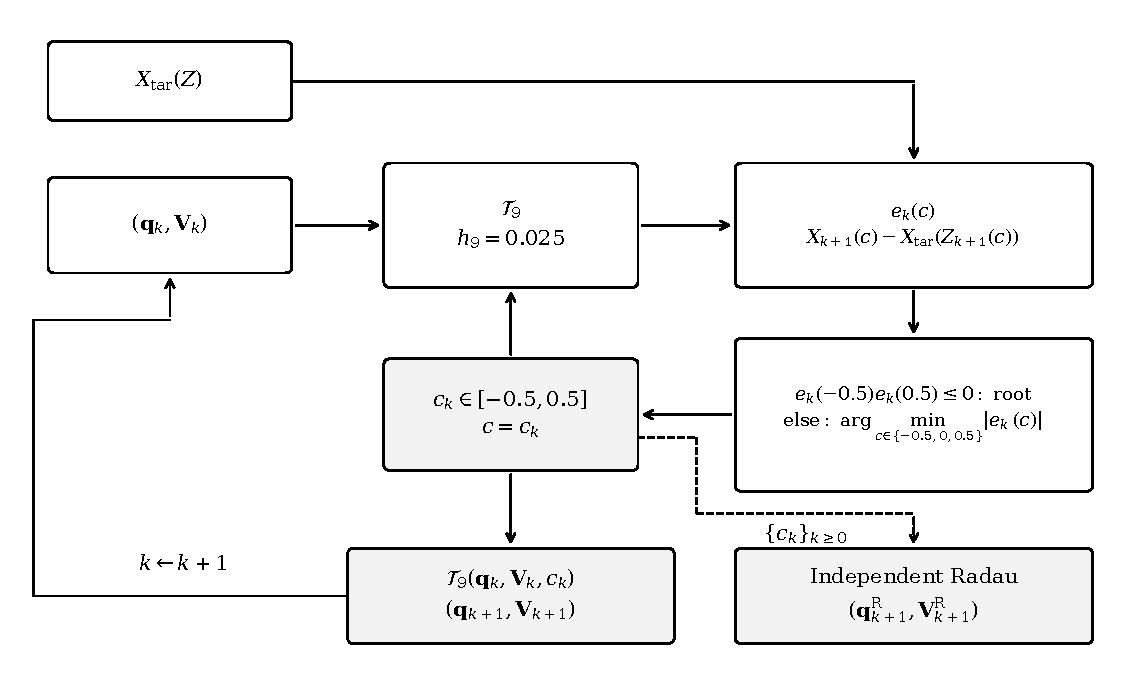
\includegraphics[width=0.9\textwidth]{figs/inverse-magnetic-master9.pdf}
\caption{انتخاب گام‌به‌گام تحریک مؤثر و بازپخش مستقل در مدل نهم.}
\label{fig:inverse-magnetic-master9}
\end{figure}

\textbf{بازیابی دو تابع تحریک در مدل دهم.}
در این روش، موقعیت‌های زمان‌دار ذره دادهٔ مسئله هستند.
جریان حامل، پارامترهای ذره و موقعیت اولیه معلوم فرض می‌شوند.
هندسه و مقیاس‌ها مطابق بخش~\ref{sec:forward-magnetic-operator} انتخاب می‌شوند.
مجهول‌ها دامنه‌های دو منبع در تعداد محدودی گرهٔ زمانی بی‌بعد هستند.
بین گره‌ها از درون‌یابی خطی استفاده می‌شود.
مسیر نامزد با اپراتور پنجره‌ای و وزن‌های ثابت ساخته می‌شود.

تابع هدف، خطای مسیر و نوسان تحریک را جریمه می‌کند.
$N$ تعداد مشاهدات زمان‌دار است.
قید دامنه برای هر دو تحریک هم‌زمان اعمال می‌شود.
$\mathbf a_j$ بردار دو دامنه در گرهٔ زمانی $\tau_j$ است.
$\mathbf W$ وزن نسبی خطای دو مختصه را تعیین می‌کند.

\begin{equation}
\begin{aligned}
\min_{\{\mathbf a_j\}}\quad
&\frac1N\sum_{k=1}^{N}
\left\|\mathbf W
 \big[\mathbf q_\theta(\tau_k^{\mathrm{obs}};\mathbf a)
 -\mathbf q_{\mathrm{obs},k}\big]\right\|^2\\
&\quad+\lambda_a\sum_j
\frac{\|\mathbf a_{j+1}-\mathbf a_j\|^2}{\tau_{j+1}-\tau_j},\\
\text{با قید}\quad
&|a_{L,j}|+|a_{R,j}|\le\sqrt{0.5}\qquad\forall j .
\end{aligned}
\label{eq:inverse-master10-proposed-objective}
\end{equation}

برازش اصلی فقط از موقعیت‌ها استفاده می‌کند.
در حالت پایه، هفت گره شامل دو انتهای بازه هستند.
وزن‌های شبکه در همهٔ برازش‌ها ثابت می‌مانند.
پنجرهٔ ثابت بی‌بعد برابر $0.0125$ است.
گرادیان حالت بین پنجره‌ها حفظ می‌شود.
متغیرهای $p_j=a_{L,j}+a_{R,j}$ و $m_j=a_{L,j}-a_{R,j}$ بهینه می‌شوند.
هر دو متغیر در بازهٔ $[-\sqrt{0.5},\sqrt{0.5}]$ قرار دارند.
این تبدیل، قید دامنه را روی تمام قطعه‌های خطی حفظ می‌کند.
بهینه‌سازی با روش محدود \lr{L-BFGS-B} و شروع‌های غیرصفر انجام می‌شود.
مسیرهای خارج از دامنه برای جواب نهایی پذیرفته نمی‌شوند.
جریمهٔ دامنه در ارزیابی نامزدها جداگانه ثبت می‌شود.
ضرایب خام تخمینی با حل‌گر مستقل بازپخش می‌شوند.

طبق رابطهٔ~\eqref{eq:forward-mag-force}، نیرو به مربع بزرگی میدان وابسته است.
تغییر هم‌زمان علامت دو تحریک، میدان را معکوس می‌کند.
نیرو و مسیرِ حاصل از معادلهٔ فیزیکی ثابت می‌مانند.
در آزمون تک‌منبعی، فعال‌بودن منبع چپ و علامت مثبت معلوم‌اند.
در آزمون دومنبعی، علامت کلی از مشاهدات معلوم فرض نمی‌شود.
ترجیح علامتِ شبکه، شاهد تعیین‌پذیری فیزیکی محسوب نمی‌شود.
پس از فاصلهٔ مشترک صفر، ابهام علامت مستقل نیز ممکن است.
تعیین‌پذیری سایر مؤلفه‌های تحریک به اطلاعات مسیر وابسته است.
خطای بازتولید مسیر و خطای بازیابی تحریک جداگانه سنجیده می‌شوند.
این صورت‌بندی در آزمایش‌های فصل نتایج استفاده شده است.

\قسمت{روش اعتبارسنجی و معیارهای ارزیابی}
\label{sec:theory-validation-metrics}

برای هر مسئله، خروجی محاسبه‌شده با یک مرجع عددی مقایسه می‌شود.
مقادیر مرجع و پیش‌بینی پیش از مقایسه با یک مقیاس بی‌بعد می‌شوند.
برای خطای نسبی، مرجع باید روی همان نقاط ارزیابی شده باشد.
نرم گسستهٔ $\|\cdot\|_{2,S}$ روی مجموعهٔ نقاط $S$ محاسبه می‌شود.

\begin{equation}
E_2(\widehat g,g;S)=
\frac{\|\widehat g-g\|_{2,S}}{\|g\|_{2,S}},
\qquad
\|g\|_{2,S}^2=\sum_{j\in S}\|g_j\|^2.
\label{eq:validation-relative-l2}
\end{equation}

این تعریف برای مرجع با نرم غیرصفر به کار می‌رود.
مقادیر خطا و تفسیر آن‌ها در فصل نتایج گزارش می‌شوند.

\textbf{بازپخش آرایش ذرات.}
بازپخش مستقل برای چهار برنامهٔ ذخیره‌شدهٔ آرایش اردک انجام شد.
برنامهٔ رهاسازی و وزن‌های شبکه در هر بازپخش ثابت ماندند.
مسیرهای میدان شبکه با \lr{RK45} محاسبه شدند.
مسیرهای مرجع با میدان تحلیلی پوازوی و \lr{DOP853} محاسبه شدند.
در هر دو حل، درگ و شرایط اولیهٔ ذرات یکسان‌اند.

بیشینهٔ خطای نهایی برای هر میدان در زمان هدف محاسبه می‌شود.
کمینهٔ فاصلهٔ مراکز در بازهٔ حضور هم‌زمان هر جفت بررسی می‌شود.
$\mathcal I_{ij}^*$ بازهٔ حضور مشترک ذرات $i$ و $j$ است.

\begin{equation}
\begin{aligned}
E_{\mathrm{target}}^*
&=\max_i\|\mathbf r_i^*(T^*)-\mathbf g_i^*\|,\\
d_{\min}^*
&=\min_{i<j}\min_{t^*\in\mathcal I_{ij}^*}
  \|\mathbf r_i^*(t^*)-\mathbf r_j^*(t^*)\|,\\
E_{\mathrm{end,diff}}^*
&=\max_i\|\mathbf r_{i,\mathrm{PINN}}^*(T^*)
           -\mathbf r_{i,\mathrm{ref}}^*(T^*)\|.
\end{aligned}
\label{eq:validation-formation-errors}
\end{equation}

کمینهٔ فاصله با نمونه‌برداری زمانی و پالایش کمینه‌های محلی برآورد شد.
حساسیت این برآورد به تعداد نمونه‌های زمانی بررسی شد.
برای نزدیک‌ترین جفت، حساسیت مکان نهایی به گام انتگرال‌گیری نیز بررسی شد.
آستانه‌های پذیرش مطابق بخش~\ref{sec:theory-particle-formation} اعمال شدند.

\textbf{عملگر مستقیم جریان.}
مرجع جریان با روش مستقل اجزای محدود ساخته شد.
شبکهٔ مثلثی در نزدیکی ورودی ریزتر است.
المان تیلور–هود از تقریب درجهٔ دوم سرعت و درجهٔ اول فشار استفاده می‌کند.
مرجع و شبکه با شرایط مرزی یکسان در نقاط مشترک مقایسه شدند.
برای فشار، هیچ جابه‌جایی پس از محاسبه اعمال نشد.

خطای نسبی بردار سرعت، مؤلفهٔ عرضی و فشار جداگانه محاسبه شد.
برای مؤلفهٔ عرضی، ریشهٔ میانگین مربعات خطای مطلق نیز گزارش می‌شود.
در ارزیاب، مخرج خطای نسبی عرضی و فشار حد پایین دارد.
این حد از تقسیم بر نرم بسیار کوچک جلوگیری می‌کند.

\begin{equation}
\begin{aligned}
E_{v,\mathrm{rms}}^*
&=\left[\frac1N\sum_{j=1}^N(\widehat v_j^*-v_j^*)^2\right]^{1/2},\\
E_{\mathrm{mom,rms}}^*
&=\left[\frac1M\sum_{j=1}^M
 \|\mathbf R_{\mathrm{NS}}^*(\mathbf x_j^*)\|^2\right]^{1/2}.
\end{aligned}
\label{eq:validation-forward-flow-rms}
\end{equation}

باقیماندهٔ مومنتوم از معادلهٔ بی‌بعد~\eqref{eq:forward-flow-equations} محاسبه می‌شود.
$N$ تعداد نقاط مشترک میدان و $M$ تعداد نقاط ارزیابی مومنتوم است.
وزن‌دهی ویژهٔ تابع هزینهٔ آموزش در این معیار اعمال نمی‌شود.
پیوستگی، شرط خروجی، پروفایل ورودی و خطای دبی نیز بررسی شدند.
مرجع‌های تکرارشونده در انتخاب وزن‌های شبکه به کار رفتند.
مرجع‌های رزروشده برای آزمون نهایی در این اجرا ارزیابی نشدند.

\textbf{عملگر مستقیم مغناطیسی.}
مرجع مسیر با انتگرال‌گیری مستقل معادلهٔ بیش‌میرا و \lr{DOP853} ساخته شد.
صحت محاسبهٔ نیرو با فرم مستقل پتانسیل مختلط بررسی شد.
در آزمون محلی، هر دو حل از تحریک درون‌یابی‌شدهٔ یکسان استفاده کردند.
در آزمون مسیر کامل، حل مرجع تابع اصلی تحریک را دریافت کرد.
مسیرهای پیش‌بینی و مرجع در زمان‌های یکسان مقایسه شدند.
خطای عرضی با $R$ و خطای محوری با $D$ بی‌بعد می‌شود.

\begin{equation}
E_{X,\infty}=\max_k|\widehat X_k-X_{\mathrm{ref},k}|,
\qquad
E_{Z,\infty}=\max_k|\widehat Z_k-Z_{\mathrm{ref},k}|.
\label{eq:validation-forward-magnetic-errors}
\end{equation}

این دو مؤلفه جداگانه گزارش می‌شوند.
در یک آزمون جداگانه، اثر تقریب بیش‌میرا بر مکان ذره بررسی شد.
در آن آزمون، مسیر بیش‌میرا با حل اینرسی‌دار \lr{Radau} مقایسه شد.

\textbf{بازسازی جریان از مسیر ذرات.}
در مثال‌های زمان‌دار، دادهٔ مصنوعی از رهگیری ذرات در میدان مرجع ساخته شد.
میدان مرجع با روش مستقل اجزای محدود به دست آمد.
از داده‌های مرجع، تنها مسیر ذرات وارد برازش شد.
پس از برازش، مسیرها با حل مستقل معادلهٔ حرکت بازپخش شدند.
خطای بازپخش در زمان‌های مشاهده محاسبه می‌شود.
برای مسیر $i$، معیارهای مکانی روی $N_i$ نقطهٔ مشترک تعریف می‌شوند.

\begin{equation}
\begin{aligned}
\Delta\mathbf r_{i,k}^*
&=\mathbf r_{i,\mathrm{replay}}^*(t_{i,k}^*)
 -\mathbf r_{i,\mathrm{obs}}^*(t_{i,k}^*),\\
E_{i,\mathrm{rms}}^*
&=\left[\frac1{2N_i}\sum_{k=1}^{N_i}
 \|\Delta\mathbf r_{i,k}^*\|^2\right]^{1/2},\\
E_{i,\max}^*&=\max_k\|\Delta\mathbf r_{i,k}^*\|.
\end{aligned}
\label{eq:validation-inverse-timed-path}
\end{equation}

عامل دو از میانگین‌گیری روی دو مؤلفهٔ مکانی می‌آید.
وضعیت تکمیل مسیر همراه خطای بازپخش گزارش می‌شود.
خطای نسبی پروفایل ورودی با سرعت مرجع مشترک محاسبه می‌شود.
در آزمون تعداد ذرات، نرم نسبی روی $4097$ نمونهٔ ارتفاعی محاسبه شد.
خطای میدان سرعت و فشار نیز روی شبکهٔ مرجع جداگانه محاسبه می‌شود.

در حالت بدون زمان، بازپخش در افق زمانی تخمینی انجام می‌شود.
هر دو روش با معیارهای هندسی مشترک مقایسه می‌شوند.
این معیارها در رابطهٔ~\eqref{eq:inverse-flow-geometry-errors} تعریف شده‌اند.
فاصلهٔ بیشینهٔ هندسی نیز با معیار هاوسدورف سنجیده می‌شود.
در همان نمادگذاری، برآورد گسستهٔ این معیار به‌صورت زیر است.
\[
E_{\mathrm H}^*=
\max\!\left\{
\max_j d(\mathbf p_j,\mathcal Q),
\max_j d(\mathbf q_j,\mathcal P)
\right\}.
\]
در گزارش فعلی، پروفایل زمان‌دار مبنای مقایسهٔ دو تخمین است.
اختلاف شکل پروفایل پس از نرمال‌سازی با میانگین هر پاسخ محاسبه می‌شود.
مقایسه با مقدار حقیقی فقط در صورت وجود مرجع معلوم گزارش می‌شود.
زمان حقیقی صرفاً پس از برازش برای مقایسهٔ مدت مسیر استفاده شد.

\textbf{رهگیری مغناطیسی مسیر هدف.}
در مدل نهم، همان تحریک مؤثر در حل‌گر مستقل \lr{Radau} بازپخش شد.
خطای رهگیری با مختصات محوری مسیر بازپخش محاسبه می‌شود.
$\mathbf q_{\mathrm{ref},k}$ حالت مکانی بازپخش در گام $k$ است.

\begin{equation}
E_{\mathrm{track},\infty}
=\max_k
 |X_{\mathrm{ref},k}-X_{\mathrm{tar}}(Z_{\mathrm{ref},k})|.
\label{eq:validation-master9-tracking}
\end{equation}

اختلاف محوری و عرضی دو حل نیز در زمان‌های یکسان محاسبه می‌شود.
وضعیت رسیدن به انتهای مسیر هدف همراه این خطاها گزارش می‌شود.

\textbf{ارزیابی بازیابی دو تحریک مغناطیسی.}
برای آزمون مصنوعی، دو تحریک مجاز و معلوم انتخاب شدند.
مسیر مرجع با حل مستقل معادلهٔ حرکت تولید شد.
نمونه‌های موقعیت مرجع به مسئلهٔ معکوس داده شدند.
برازش با اپراتور ثابت و تابع هدف بخش~\ref{sec:inverse-magnetic-drive} انجام شد.
تحریک تخمینی با همان حل‌گر مستقل بازپخش شد.
خطای مسیر بازپخش با معیارهای رابطهٔ~\eqref{eq:validation-forward-magnetic-errors} سنجیده شد.

خطای تحریک روی شبکهٔ زمانی مشترک با مرجع محاسبه شد.
در این مقایسه، قرارداد علامت برای هر دو پاسخ یکسان است.
اگر علامت مشخص نباشد، دو علامت کلی در مقایسه بررسی می‌شوند.
برای تحریک مرجع صفر، فقط خطای مطلق گزارش می‌شود.

\begin{equation}
E_a=
\min_{\sigma\in\Sigma}
\frac{\|\widehat{\mathbf a}-\sigma\mathbf a_{\mathrm{ref}}\|_{2,S}}
{\|\mathbf a_{\mathrm{ref}}\|_{2,S}},
\qquad
\Sigma=
\begin{cases}
\{+1\}, & \text{علامت معلوم},\\
\{-1,+1\}, & \text{علامت نامعلوم}.
\end{cases}
\label{eq:validation-master10-proposed-recovery}
\end{equation}

خطاهای دامنهٔ هر منبع نیز جداگانه بررسی شدند.
در صورت نیاز، میدان و نیرو در نقاط مشترک مقایسه شدند.
زمان‌های مشاهدات و ارزیابی مستقل، شبکه‌های جداگانه دارند.
شرط اولیه در آزمون‌های نویزی دقیق نگه داشته شد.
مقیاس خطا، بیشینهٔ نویز معلوم و کف خطای عملگر است.
کف عرضی $5.5\times10^{-5}$ و کف محوری $4\times10^{-5}$ است.
این کف‌ها پیش از برازش از ارزیابی مستقیم تعیین شدند.
ضریب پایهٔ جریمهٔ زبری $\lambda_a=0.1$ است.
حساسیت به وزن، زبری، گره‌ها و پنجره نیز بررسی شد.
همگرایی بهینه‌ساز و دقت بازیابی تحریک جداگانه گزارش می‌شوند.

جدول~\ref{tab:validation-summary} مرجع و معیار اصلی هر مطالعه را خلاصه می‌کند.

\begin{table}[htbp]
\centering
\small
\caption{مرجع عددی و معیارهای بی‌بعد ارزیابی هر مطالعه.}
\label{tab:validation-summary}
\begin{tabular}{@{}p{0.24\linewidth}p{0.29\linewidth}p{0.40\linewidth}@{}}
\hline
\textbf{مطالعه} & \textbf{مرجع مقایسه} & \textbf{معیار اصلی}\\
\hline
آرایش ذرات &
بازپخش با میدان تحلیلی پوازوی &
خطای مکان نهایی، اختلاف دو بازپخش و کمینهٔ فاصله\\
عملگر مستقیم جریان &
حل مستقل اجزای محدود &
خطای سرعت، مؤلفهٔ عرضی و فشار، باقیماندهٔ مومنتوم\\
عملگر مستقیم مغناطیسی &
حل مستقل معادلهٔ بیش‌میرا &
بیشینهٔ خطای عرضی و محوری\\
بازسازی جریان زمان‌دار &
مشاهدات مسیر و میدان مرجع &
خطای بازپخش، پروفایل ورودی و میدان\\
بازسازی جریان بدون زمان &
هندسهٔ مشاهده‌شده و تخمین زمان‌دار &
فاصلهٔ هندسی مسیر و اختلاف دو پروفایل\\
رهگیری مغناطیسی مدل نهم &
بازپخش مستقل و مسیر هدف &
خطای عرضی رهگیری و اختلاف دو حل\\
بازیابی دو تحریک مغناطیسی &
تحریک معلوم و مسیر مرجع مصنوعی &
خطای بازیابی تحریک و بازپخش مستقل مسیر\\
\hline
\end{tabular}
\end{table}
